\section{Implementation}
\subsection{Parallel radix-$2^3$ 16-Points}
\begin{frame}
  \frametitle{\textbf{Table of Contents}}
  \begin{center}
    {\vspace{-1.5cm}\Large \textbf{Sección \thesection}\vspace{0.5cm}}
    \begin{beamercolorbox}[
      sep=8pt,center]{part title}
      \usebeamerfont{part title}
      \textbf{\insertsection}
    \end{beamercolorbox}
  \end{center}
\end{frame}


\begin{frame}
	\frametitle{\textbf{Design of FFT architecture via folding transformation}}
	\framesubtitle{\secname : \subsecname}
	%\vspace{-0.5cm}
		\begin{figure}[h!] \centering
		   	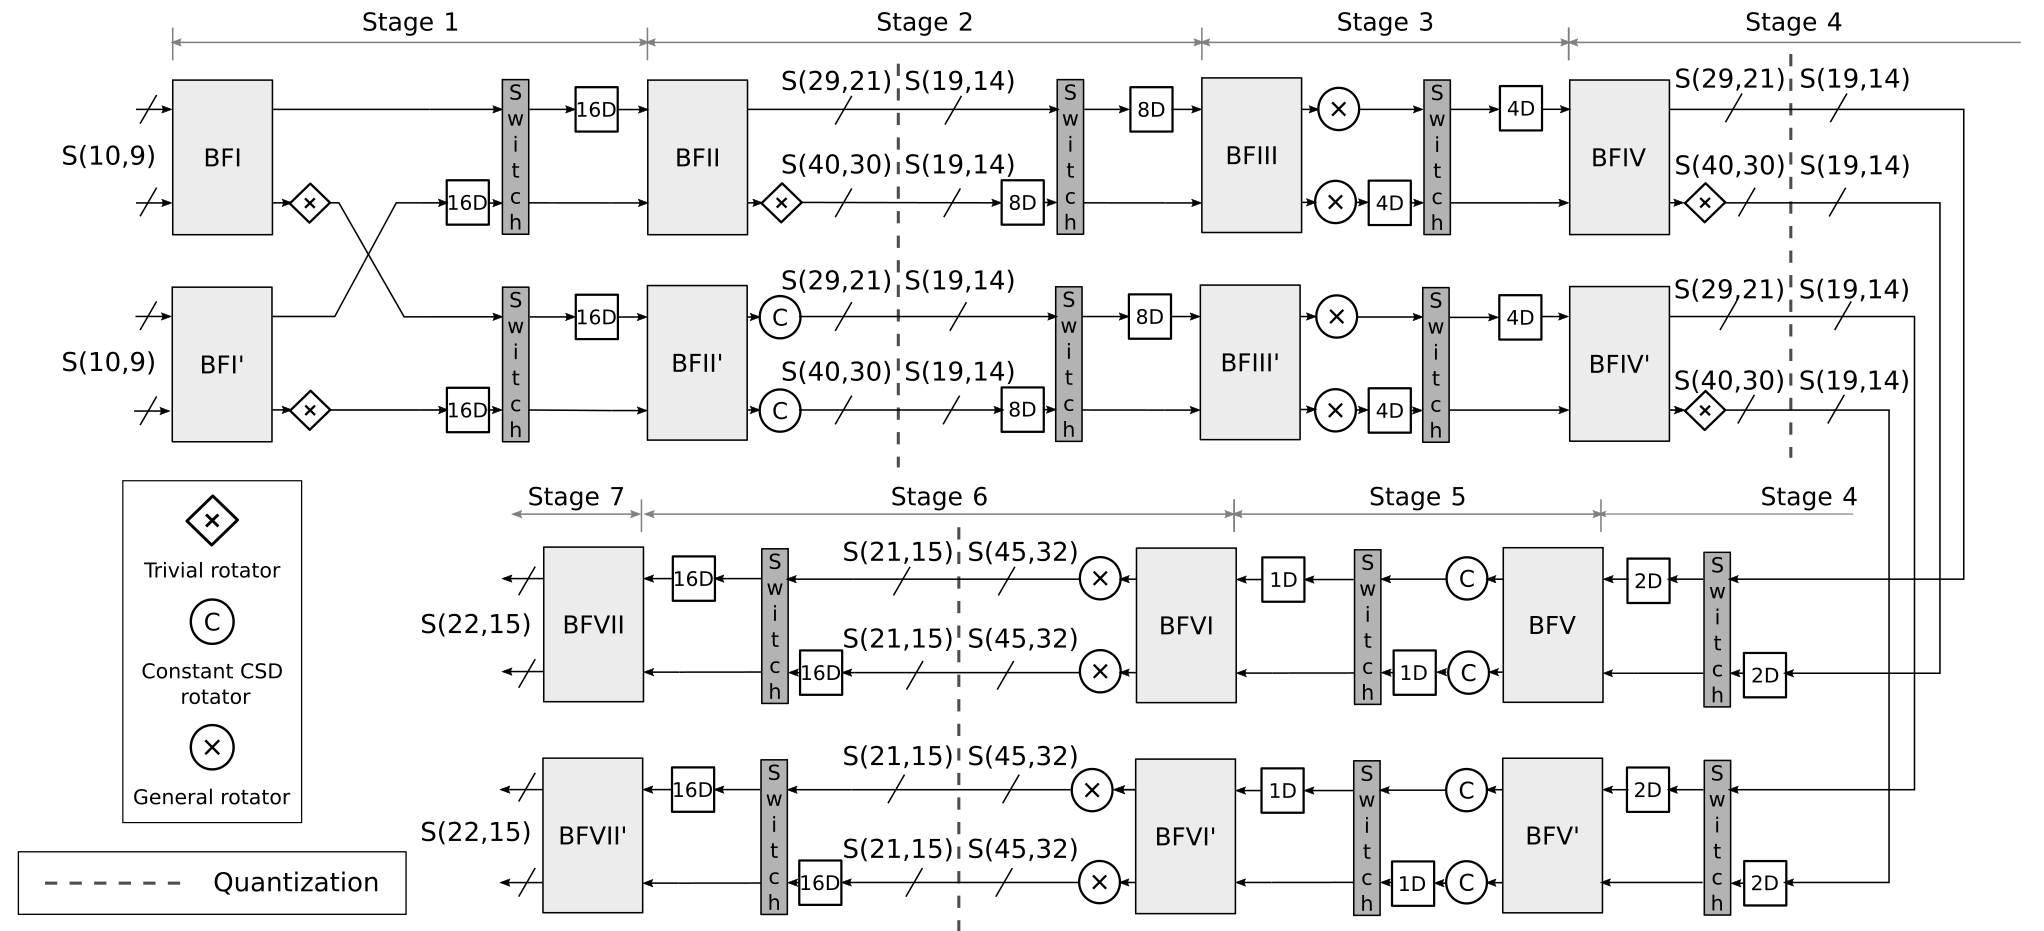
\includegraphics[width=0.90\paperwidth]{./image/folding-128-quant.png}
		   	\caption{ \tiny Folding architecture for radix-$2^3$  128 points FFT with quatization.}
		\end{figure}  	
\end{frame}


\begin{frame}
	\frametitle{\textbf{Design of FFT architecture via folding transformation}}
	\framesubtitle{\secname : \subsecname}
	\vspace{-0.5cm}
	%\begin{block}{\centering }
	%We can deduce the folding architecture for 128 points following the same method. 
	%\end{block}
		\begin{figure}[h!] \centering
		   	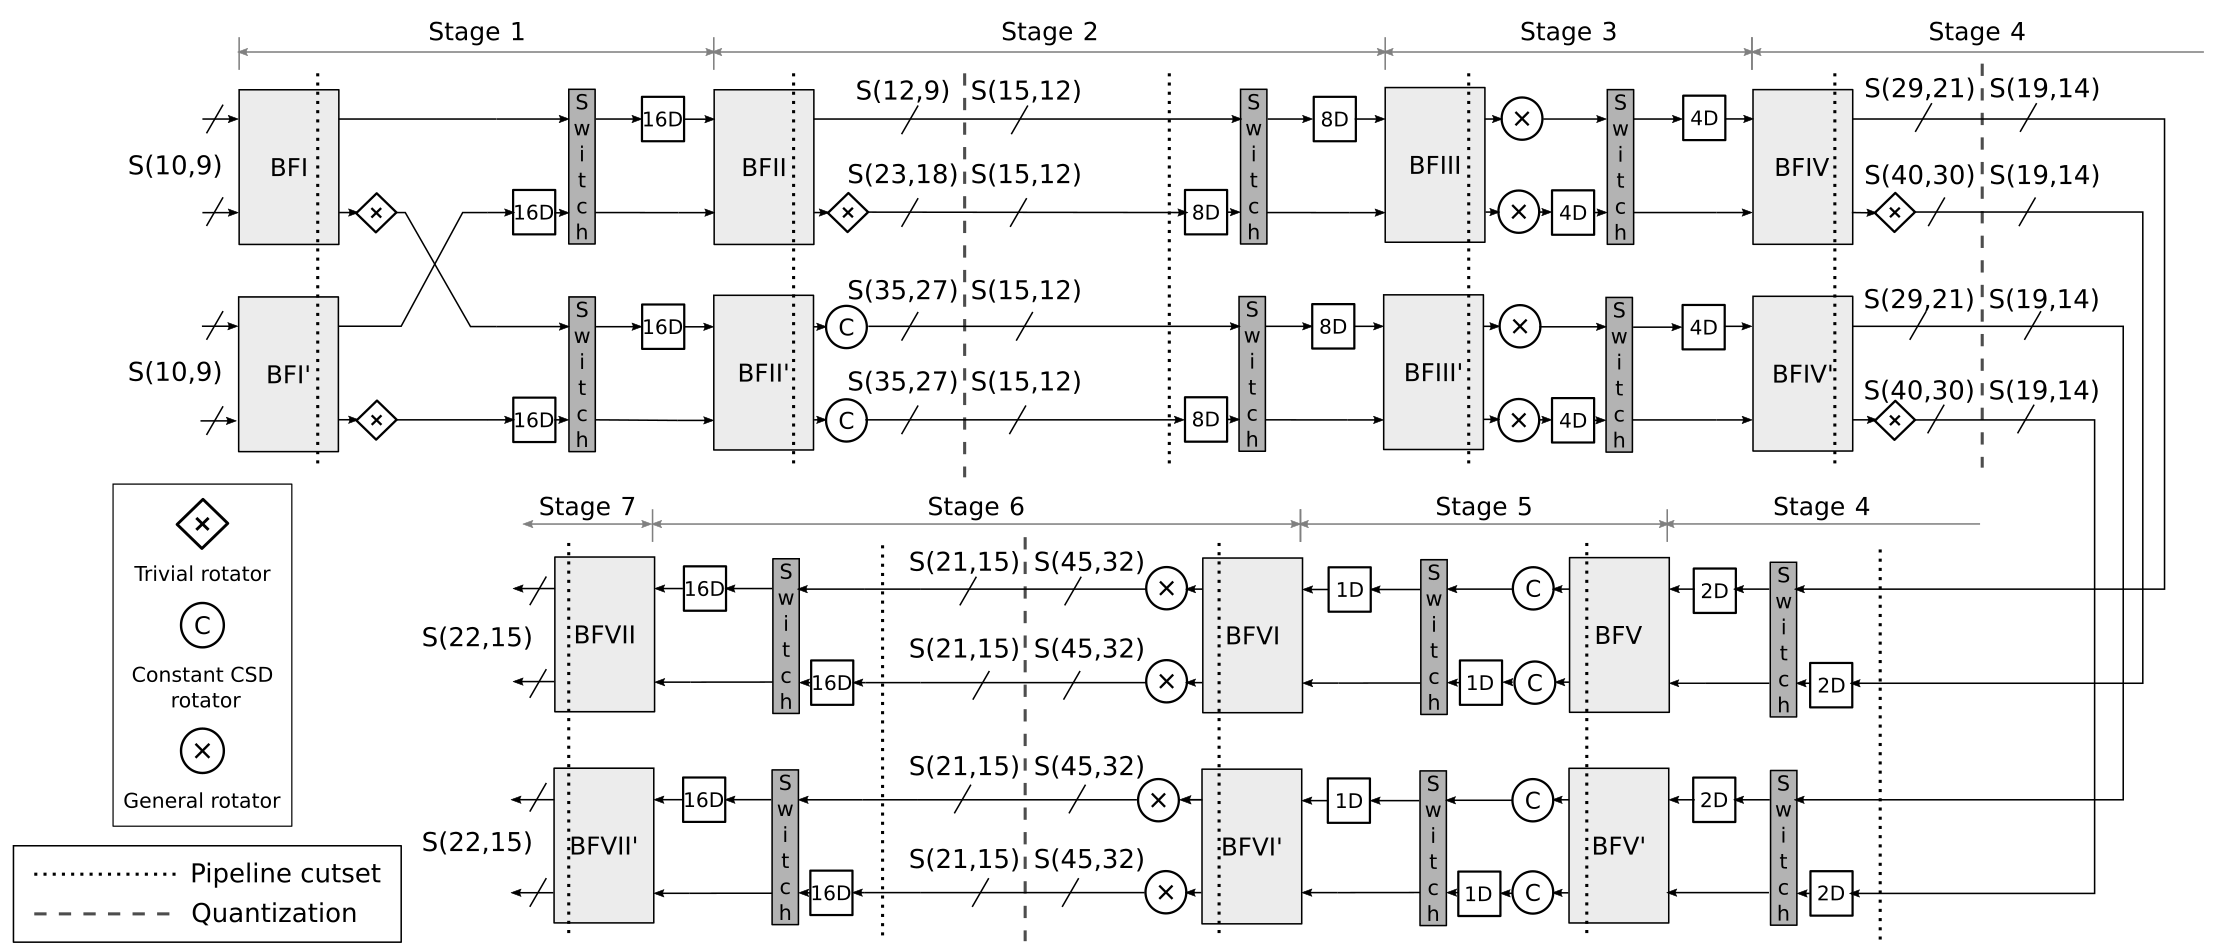
\includegraphics[width=0.95\paperwidth]{./image/folding-128-quant-pipe.png}
		   	\caption{ \tiny Folding architecture for radix-$2^3$ 128 points FFT with quantization and pipeline.}
		\end{figure}  	
\end{frame}